%%%%%%%%%%%%%%%%%%%%%%% file template.tex %%%%%%%%%%%%%%%%%%%%%%%%%
%
% This is a general template file for the LaTeX package SVJour3
% for Springer journals.          Springer Heidelberg 2010/09/16
%
% Copy it to a new file with a new name and use it as the basis
% for your article. Delete % signs as needed.
%
% This template includes a few options for different layouts and
% content for various journals. Please consult a previous issue of
% your journal as needed.
%
%%%%%%%%%%%%%%%%%%%%%%%%%%%%%%%%%%%%%%%%%%%%%%%%%%%%%%%%%%%%%%%%%%%
%
% First comes an example EPS file -- just ignore it and
% proceed on the \documentclass line
% your LaTeX will extract the file if required
%\begin{filecontents*}{example.eps}
%!PS-Adobe-3.0 EPSF-3.0
%%BoundingBox: 19 19 221 221
%%CreationDate: Mon Sep 29 1997
%%Creator: programmed by hand (JK)
%%EndComments
%gsave
%newpath
 % 20 20 moveto
  %20 220 lineto
  %220 220 lineto
  %220 20 lineto
%closepath
%2 setlinewidth
%gsave
%  .4 setgray fill
%grestore
%stroke
%grestore
%\end{filecontents*}
%
\RequirePackage{fix-cm}
%
%\documentclass{svjour3}                     % onecolumn (standard format)
\documentclass[smallcondensed]{svjour3}     % onecolumn (ditto)
%\documentclass[smallextended]{svjour3}       % onecolumn (second format)
%\documentclass[twocolumn]{svjour3}          % twocolumn
%
\smartqed  % flush right qed marks, e.g. at end of proof
%
\usepackage{graphicx}
%
% \usepackage{mathptmx}      % use Times fonts if available on your TeX system
%
% insert here the call for the packages your document requires
%\usepackage{latexsym}
\usepackage{algorithm}
\usepackage{algorithmicx}
\usepackage{algpseudocode}
%\usepackage{amsmath}
\usepackage{amssymb, amsmath}
\usepackage{footmisc}
%\usepackage{amsthm}
\usepackage{graphicx}
\usepackage{subfigure}
%\usepackage{caption2}
\usepackage{indentfirst}
%\captionsetup{belowskip=-17pt}
% etc.
%
% please place your own definitions here and don't use \def but
% \newcommand{}{}
%\newtheorem{definition}{Definition}
%\newtheorem{theorem}{Theorem}
% Insert the name of "your journal" with
% \journalname{myjournal}
%
\begin{document}
\title{Time-Bounded Positive Influence in Social Networks}
%\subtitle{Do you have a subtitle?\\ If so, write it here}

%\titlerunning{Short form of title}        % if too long for running head

\author{Tuo Shi   \and
        Siyao Cheng \and
        Zhipeng Cai \and
        Yingshu Li \and
        Jianzhong Li %etc.
}

%\authorrunning{Short form of author list} % if too long for running head
\institute{Tuo Shi \at
              Harbin Institute of Technology \\
              %Tel.: +123-45-678910\\
              %Fax: +123-45-678910\\
              \email{shituo@hit.edu.cn}           %  \\
%             \emph{Present address:} of F. Author  %  if needed
           \and
           Siyao Cheng \at
              Harbin Institute of Technology\\
              \email{csy@hit.edu.cn}
		  \and
		  Zhipeng Cai\at
		    Georgia State University\\
		    \email{zcai@cs.gsu.edu}
		   \and
		Yingshu Li\at
			Georgia State University\\
			\email{yili@cs.gsu.edu}
			\and
		Jianzhong Li\at
			Harbin Institute of Technology\\
			\email{lijzh@hit.edu.cn}
}

\date{Received: date / Accepted: date}
% The correct dates will be entered by the editor
\maketitle
\begin{abstract}
The appearance of social networks provides great opportunities for people to communicate, share and disseminate information. Meanwhile, it is quite challenge for utilizing a social networks efficiently in order to increase the commercial profit or alleviate social problems. One feasible solution is to select a subset of individuals that can positively influence the maximum other ones in the given social network, and some algorithms have been proposed to solve the optimal individual subset selection problem. However, most of the existing works ignored the constraint on time. They either assume that the time is infinite or only suitable to solve the snapshot selection problems. Obviously, both of them are impractical in the real system. Due to such reason, we study the problem of selecting the optimal individual subset to diffuse the positive influence when time is bounded. We proved that such a problem is NP-hard, and a heuristic algorithm based on greedy strategy is proposed. The experimental results on both simulation and real-world social networks based on the trace data in Shanghai show that our proposed algorithm outperforms the existing algorithms significantly, especially when the network structure is sparse.
\keywords{social network \and influence \and dominating set}
% \PACS{PACS code1 \and PACS code2 \and more}
% \subclass{MSC code1 \and MSC code2 \and more}
\end{abstract}

\section{Introduction}
\label{intro}
Social network is a platform consisting of individuals who share same interests, activities and backgrounds or have real-life connections.
With the exponential growth of online social networks, more and more people are involved. According to the recent statistics, there are more than a billion Facebook accounts in the world.
Among the billions of online social network individuals, more than 27\% and 40\% Europeans access social networks at least once within a day and a week,
respectively \cite{Think2014}.
Such a platform provides great opportunities for people to communicate, share and disseminate information.
The popularity of social networks and their influences among individuals have attracted a great deal of attention due to its great
potential benefits on both economy and society \cite{ShiNew/WLZC2015}	 .
For example, in viral marketing, commercial companies can utilize social network as a channel to publicize their products \cite{ShiNew/WCDD2015}.
Many intervention and education programs take advantage of this platform to help with alleviating social problems, such as drinking, smoking and drug problems. The government can also use social networks to stop rumors \cite{ShiNew/HCW2015}\cite{ShiNew/WCGP2015} . 

In general, a social network can be represented as a graph $G(V, E)$, where $V$ is the set of nodes representing the individuals in a social network,
$E$ is the set of edges where each edge represents the social tie between two individuals.
Many research works indicate that individuals have tendency to follow the behaviors of their friends and relatives rather than the information obtained from other ways,
such as radio, TV and online advertisement \cite{JBD2005}, and this tendency is growing with the increase of the number of her friends having the same behavior.
Thus, one promising way to take advantage of social networks is to select a subset of individuals to positively influence other nodes in a social network, that is,
this subset is expected to result in large cascade of further adoptions.
%The problem is called influence maximization problem.
The major reason to choose a subset of individuals instead of nodes in a whole network is because of budget limitation which is the primary concern for many applications.
For example, a commercial company can promote some individuals in a social network with a fixed budget and ask them to publicize their products.
An intervention program can select a subset of binge drinkers to participate such that they will positively influence other binge drinkers subsequently
over a social network.
The government can also depend on a subset of individuals to spread the truth in order to stop rumors.
%The problem has been formulated into some discrete optimization problems with different object functions and constraints recently.
%For example, Kempe {\it et al.} \cite{KKT2003} proposed a first influence maximization problem, which is to select a fix number of candidates such that the
%expected influence node become maximal.
%The algorithm is further improved by quite a few works \cite{LKG2007,CWY2009,WCW2012} in term of time complexity.
One efficient way to address the aforementioned problems is to make use of a dominating set \cite{KLA2013}.
A node set $D$ is called a dominating set of graph $G$ if each node in $G$ not in $D$ has at least one neighbor in $D$.
However, the approaches employing dominating sets only consider individual-to-individual social influence, which is not practical in social networks.
It is indicated by \cite{JBD2005} that positive (negative) influence from more neighbors/friends will result in more impact to an individual.
That is, if one individual will turn from negative to positive with a high probability if she has more positive friends than negative friends.
Wang {\it et al.} \cite{WDC2011} take the group-to-individual interaction into account and introduce a more reasonable model in social networks.
They studied the Positive Influence Dominating Set (PIDS) problem.
A set $D$ is called a PIDS if for each individual in a social network, there are more than half of its neighbors belonging to $D$.
Wang {\it et al.} proposed a greedy approximation algorithm to derive the least possible set to influence all the nodes.
In many previous works, the problems are always formulated as discrete optimization problems (influence maximization problems) with different object functions and constraints.
For example, Kempe {\it et al.} \cite{KKT2003} proposed the first influence maximization problem, which is to select a fixed number of candidates such that the
expected number of the influenced nodes can be maximized.
However, one of the key factors, time constraint, has been overlooked by most existing studies.
The goal of the influence maximization problem is to maximize the expected number of influenced nodes after an unbounded time period,
while the purpose of the PIDS problem is to find a dominate set $D$ such that all the other nodes can be influenced by $D$ instantly.
In many real-world applications, time is an inevitable factor that needs to be considered.
For example, in viral marketing, commercial companies are expected to know the effect of popularization within a time limit in order to ensure the normal
operation of the chain of funds.
Government always wants to stop rumors within a certain time to reduce public panic.
Another factor overlooked by most of the existing works is the negative influence.
Note that people can have both positive and negative influence on their close friends in social networks
and an individual could turn back and forth with the changing of her neighbors.
For example, one can trust the truth at the beginning and will have positive impact on her direct friends, on the other hand, she may believe the rumors if most of her friends pass negative information to her.

Motivated by the aforementioned factors, we consider the problem of how to select as few initial users as possible to influence all of the users
in a social network within a certain time limit in this paper.
An individual is positively influenced if more than half of its neighbors have positive impact on its and vice versa.
In this paper, we first introduce the problem of finding a time-bounded Positive Influence Dominating Set (tPIDS), and propose a greedy algorithm to find the smallest possible size of a subset of the nodes in a social network which can
influence the whole network within time $t$, where $t$ is a parameter specified by users.
In summary, the main contributions of this paper are summarized as follows.
\begin{enumerate}
	 \item The time-bounded Positive Influence Dominating Set problem is defined and we show finding a minimum tPIDS is NP-hard.
	 \item A greedy algorithm is proposed.The algorithm is based on the tPIDS SPREAD graph built on an original graph.
	 The Move-Down operation is defined to adjust a tPIDS in order to find a feasible solution.
	 The complexity of our greedy algorithm is also analyzed.
	 \item The correctness of our proposed algorithm is proven, that is, the solution returned by our algorithm is valid tPIDS of social networks.
	 \item We conduct extensive experiments on randomly generated graphs and real-world social networks like trace data sets provided by \cite{sju}. On loosely structured networks with roughly uniform degree of nodes, the initial influence set can be reduced by 15\%-20\% and the running time of our algorithm is acceptable. The experimental results indicate that our greedy algorithm is effective and efficient to find a tPIDS. \\
\end{enumerate}

The rest of the paper is organized as follows.
Section II summarizes the state-of-art works on the influence maximization problem.
Section III provides the problem definition.
Section IV proposes a greedy algorithm and proves that the result returned by our algorithm is feasible tPIDS of social networks.
Section V presents the experimental results.
Section VI concludes the paper.
\section{Related Works}
\label{sec:1}
Domingos and Richardson first proposed the influence maximization problem \cite{RD2002}.
The milestone work for the influence maximization problem is \cite{KKT2003}.
The problem is formulated as a discrete optimization problem which is to find $k$ most influential nodes such that the expected number of the influenced nodes by the $k$ seeds is maximized.
Two fundamental information diffusion models, the Independent Cascade (\emph{IC}) model and the Linear Threshold (\emph{LT}) model are introduced.
They first showed the problem is NP-hard and proposed two greedy algorithms with performance ratio of $1-\frac{1}{e}$ for both the IC and LT models.
The experimental results demonstrate their greedy algorithms significantly outperform two straightforward algorithms, classic degree and centrality-based heuristics.
Kimura and Saito \cite{KS2006} proposed an efficient algorithm to calculate influence spread under shortest-path based influence cascade models.
Leskovec {\it et al.} \cite{LKG2007} proposed a Cost-Effective Lazy Forward (CELF) scheme to select seeds.
CELF significantly reduces the number of evaluations on the influence spread ability of nodes by utilizing the submodularity property of the influence maximization objective.
CELF speeds up the previous greedy algorithm more than a hundred times.
Chen {\it et al.} \cite{CWY2009} further improved the CELF algorithm in terms of scalability.
They proposed an efficient heuristic algorithm which can keep the same approximation ratio but improve the running time significantly.
Liu {\it et al.} \cite{LLL2012} utilized the supervised Monte Carlo method to estimate the influence spread for nodes with specified precision by the sampling technology.
Sheldon {\it et al.} \cite{SDE2012} proposed a mixed integer programming formulation to maximize spread of cascades in networks.
Although the objective function is not submodular anymore, their proposed preprocessing techniques can significantly reduce the computation time.
Jung {\it et al.} \cite{JHC2011} proposed a novel algorithm IRIE that incorporates Influence Ranking (IR) with a fast Influence Estimation (IE) method
in order to obtain scalability and robustness.
The Independent Cascade(IC) model and its extended version, the Independent Cascade Negative (IC-N) model, were considered.
Wang {\it et al.} \cite{WCS2010} proposed a novel greedy algorithm for selecting top-K influential nodes based on the community structure of a graph.
Due to the fact that individuals within the same community have close relationships thus are more likely to influence each other while individuals among different communities
are less likely to influence each other, the community based greedy algorithm chooses influential nodes within communities.
All the aforementioned models try to maximize the expected number of the influenced nodes and do not take the time factor into account.

Another vein of the influence maximization problem is to select a positive influence dominating set.
Dominating set, a subset $D$ of node set $V$ in graph $G$ such that every node not in $D$ is adjacent to at least one member of $D$,
has been widely studied and utilized in many real life applications \cite{GWL2009}.
A positive influence dominating set is a variation of a dominating set, which is more suitable for social networks.
A PIDS is a subset of graph $G$, called $D$, such that any node $v$ in $G$ is dominated by at least $\lceil\frac{deg(v)}{2}\rceil$ nodes in $D$.
Wang {\it et al.} \cite{WDC2011} first defined the PIDS problem in general random graphs.
They proved the NP-hard of the Minimum Positive Influence Dominating Set (MPIDS) problem and proposed a greedy algorithm with approximation ratio $H(\delta)$ to construct an MPIDS
in $O(n^3)$ time, where $H$ is the harmonic function and $\delta$ is the maximum node degree.
Zhang {\it et al.} \cite{ZWW2011} investigated the MPIDS problem in power-law graphs and proposed a greedy algorithm with a constant approximation ratio.
Raei {\it et al.} \cite{CLZ2012} further improved the greedy algorithm with time complexity $O(n^2)$ for a graph with power-law degree distribution.
Dihn {\it et al.} \cite{DSN2014} extended the PIDS problem to a more general version, called the Total Positive Influence Dominating Set (TPIDS) problem.
This problem is to seek a minimum sized $D$ such that every node in a graph has a fraction $\rho$ of neighbors in $D$.
They proved a minimized TPIDS cannot be approximated with factor $1-\epsilon \ln\max \{\delta, V^\frac{1}{2}\}$ for general graphs where $\delta$ is the maximum degree in a graph.
A simple proof was provided to show the problem can be approximated within factor $\ln \delta + O(1)$.
For a power law graph, a constant factor approximation algorithm was proposed \cite{DSN2014}.
Note that, all the PIDS related problems are to seek a dominating set which can instantly affect all the nodes in a network, thus the size of a PIDS is large, which is not practical.
In this paper, we will introduce a novel positive influence dominating set formulation by taking the time limit into account.

\begin{figure}[t]
	\subfigure[An example of 2PIDS.]
	{\label{fig:example:e0}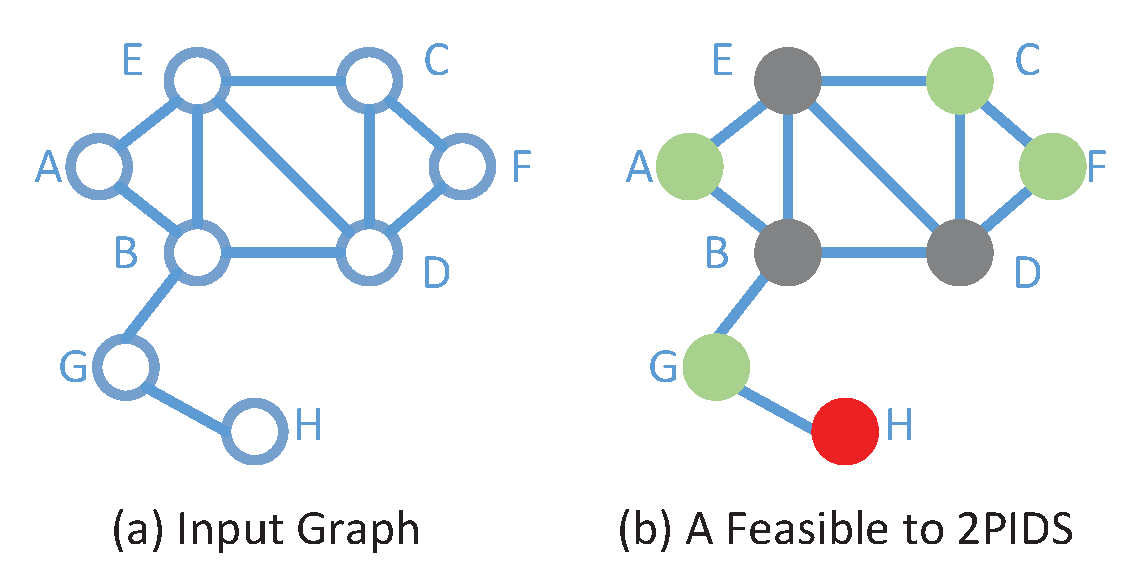
\includegraphics[width=0.5\textwidth]{Figure1.eps}}		
	%\begin{minipage}[t]{1\linewidth}
	\subfigure[The layers.]{\label{fig:example:e1}\includegraphics[width=0.24\textwidth,height=3cm ]{LayerGraph.eps}}
	\subfigure[ $t$-SPREAD graph.]{\label{fig:example:e2}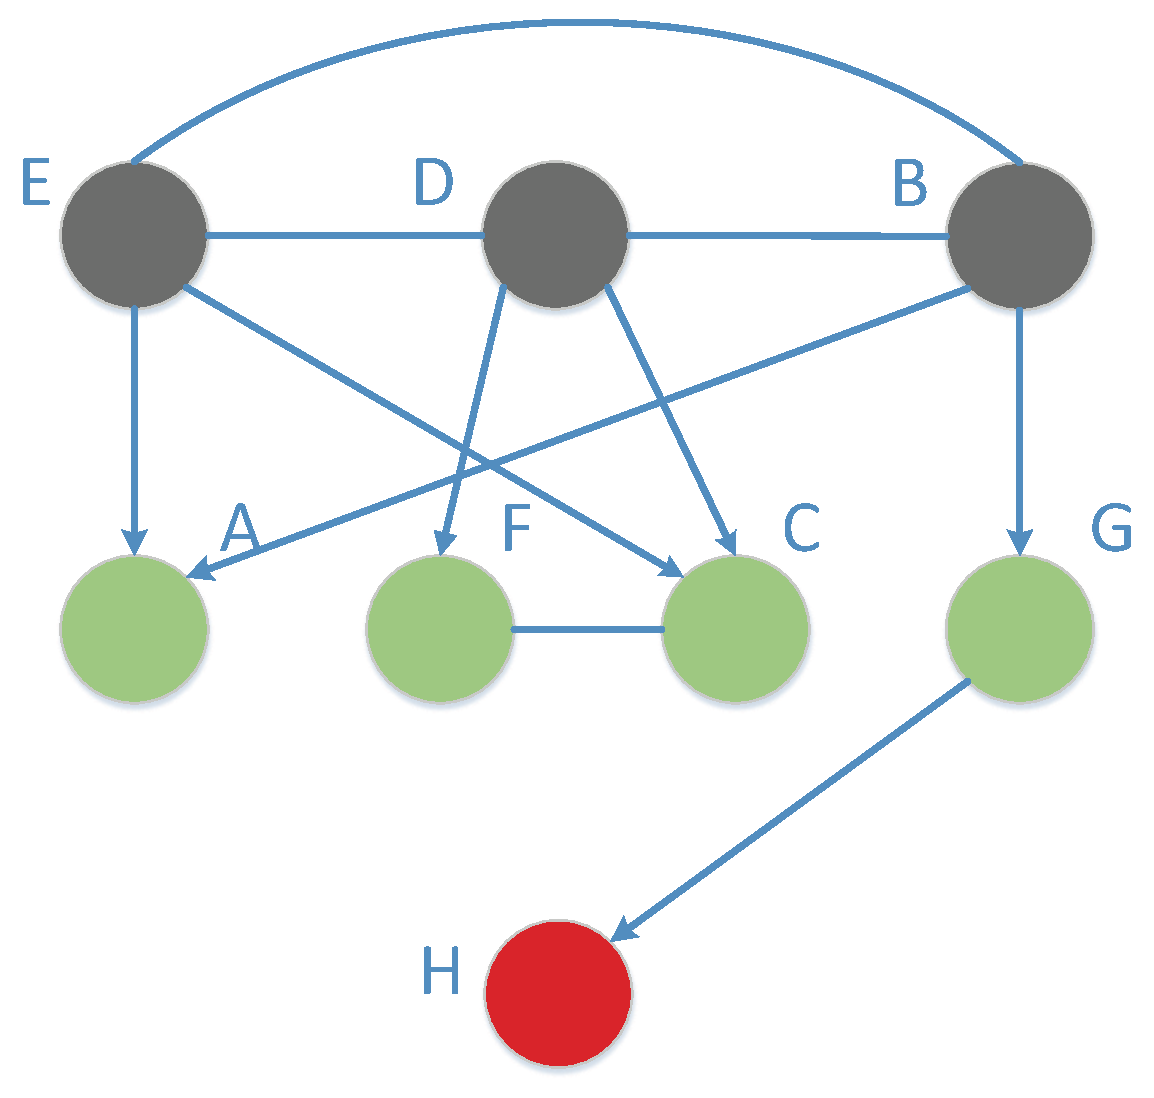
\includegraphics[width=0.24\textwidth]{Figure2.eps}}
	%\end{minipage}
	\caption{Examples}
\end{figure}
\vspace{-0.5cm}
\subsection{Problem Definition}
\label{sec:2}
Assume a social network can be represented by an undirected graph $G=(V,E)$, where $v \in V$ is an individual in the social network and $e \in E$ represents the existence of social
relationship between two individuals.
Let $deg(v)$ be the number of the neighbors of $v$.
That is, there are in total $deg(v)$ individuals who have direct social relationship with $v$.
A set $D$ is called a dominating set of $G$ if each node not in $D$ has at least one neighbor in $D$.
\begin{definition}[Positive Influence Dominating Set (PIDS)]
	Given an undirected graph $G=(V, E)$, a node $v$ is influenced by set $D$ if at least $\lceil \frac{deg(v)}{2} \rceil$ of its neighbors is in the influence set $D$.
	A set $P$ is called an influenced set of $D$ if each $v \in P$ is influenced by $D$, defined as $P \models D$.
	A set $D$ is a Positive Influence Dominating Set (PIDS) of $G$ if $V \models D$.
\end{definition}
\begin{definition}[Time-bounded Positive Influence Dominating Set (tPIDS)]
	Given an undirected graph $G=(V, E)$, a set $D_0$ is a $t$ Positive Influence Dominating Set (tPIDS) of G if
	$V \models D_{t-1} \models \cdots D_i \cdots \models D_1 \models D_0$ where $D_i \subset V$ $(1 \le i \le t-1)$ and $D_i=\arg \max |P|_{P \models D_{i-1}}$.
	That is, $D_i$ is the largest set among all the set influenced by $D_{i-1}$.
\end{definition}
Note that in a tPIDS, all the nodes influenced by $D_i$ will be included in $D_{i+1}$.
That is, $D_i \subseteq D_{i+1}$.\\
$~~~~$The goal of constructing a $tPIDS$ is to find a set $D_0$ which can positively influence the whole network within time $t$.
For example, a commercial company wants to find a group of customers to propagate the produces such that all the customers
in a social network will be positively influenced within a certain time.
An intervention program wants to educate a set of binge drinkers such that positive effect of the intervention will conquer the negative effect within a certain time.
Government wants to select a set of people in a social network to stop a rumor in
a short time.
Apparently, $V$ is the largest tPIDS of $G=(V, E)$.
However, it is costly to include all or too many individuals in a tPIDS.
Our considered problem is to find a Minimum tPIDS (MtPIDS).
That is, we want to use the least possible cost to positively influence the whole network in a certain time.
%\begin{figure}
%   \centering
%   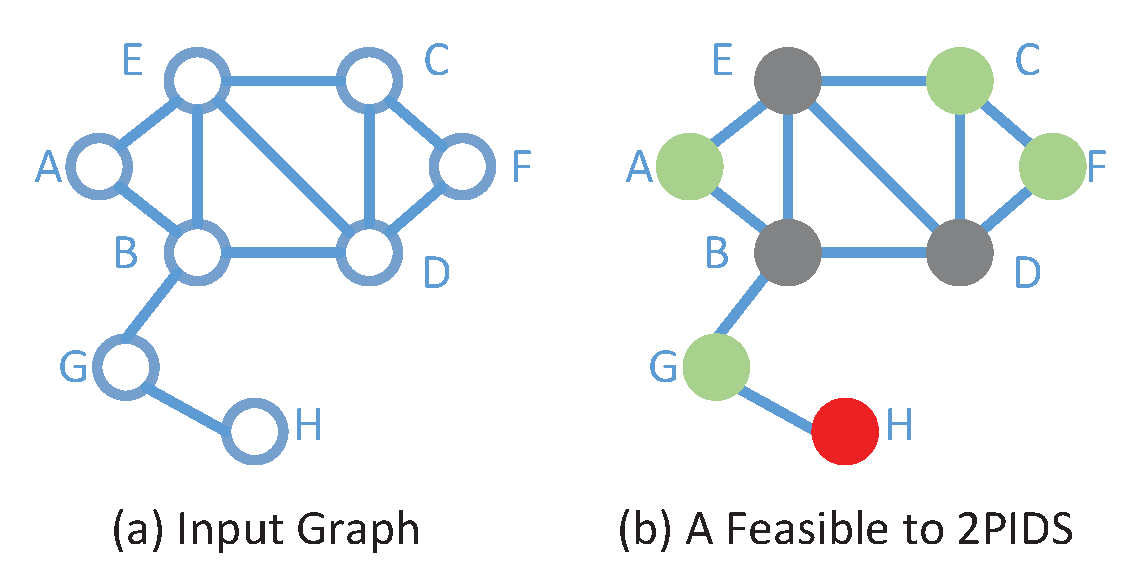
\includegraphics[width=5cm]{Figure1.eps}
%   \caption{An example 2PIDS.}
%\end{figure}
The left graph in Fig.1(a) is an input graph $G=(V , E)$ where $V = \{A ,B ,C ,D , E , F , G , H\}$.
Let $D_0 = \{B ,D ,E\}$ which is the black node set in the right graph Fig.1(a).
The green nodes $A$,$C$,$F$ and $G$ in the graph are influenced by $D_0$ and will be included in $D_1$. So $D_1=\{A ,B ,C,D , E,F ,G\}$.
The red node $H$ is influenced by $D_1$ and will be included in $D_2$. So $D_2 = \{A ,B ,C ,D , E , F , G , H\} = V$.
Thus $D_0$ is a feasible 2PIDS with size 3.
\begin{theorem}
	MtPIDS is NP-hard.
\end{theorem}

\emph{Proof:} It has been shown in \cite{WDC2011} that finding a minimum PIDS is NP-hard.
Since finding MtPIDS is a general version of finding a minimum PIDS, MtPIDS is NP-hard.
\begin{definition}[$t$-SPREAD]
	Given an influence set $D_k \subseteq V$, $D_{k+1}$ is the set with the maximum size such that $D_{k+1} \models D_k$.
	Let $L_{k+1} = D_{k+1}-D_k$,then $L_{k+1}$ is the set of influence nodes of $D_k$.
	Note that $L_0 = D_0$.
	Then the transition from $D_k$ to $D_{k+1}$ is called a SPREAD.
	Given a graph $G = (V , E)$, $G$ is said to be $t$-SPREAD to $D_0$ if $V$ can be obtained from an initial set $D_0~(D_0 \subseteq V)$ in $t$ times of SPREAD.
\end{definition}
If graph $G$ is $t$-SPREAD to $D_0$, then $V$ can be divided into $t+1$ layers (Fig.\ref{fig:example:e1}).
Let $L_0,L_1,\dots,L_t$ be the set of nodes in each layer.
For an arbitrary node $u$ in set $V$, there exists an integer $k~(0\le k\le t)$, such that $u$ belongs to set $L_k$.
Let $deg(u)$ be the degree of node $u$, and $N(u)$ be the set of neighbors of $u$.
According to the definition of tPIDS, there exists an integer $p ~(p\ge \lceil \frac{deg(u)}{2}\rceil)$ and a set $H(u)$ such that $H(u) \subseteq N(u)$, $H(u) \subseteq D_{k-1}$ and $|H(u)|=p$.
That is to say, if $u$ belongs to $L_k$, then at least half of its neighbors  are in the inner layers of $L_k$.
\begin{definition}[$t$-SPREAD graph]
	For each node $u$ in $V$, draw a directed edge from each node in $H(u)$ to $u$, an undirected edge from each node in $N(u)$ which is in the same layer with $u$ to $u$ and a directed edge from $u$ to the rest of the nodes in $N(u)$ to form a $t$-SPREAD graph.
\end{definition}
An example of $t$-SPREAD graph based on the graph in Fig.1(a) is shown on Fig.\ref{fig:example:e2}.
For each node $u$ in a $t$-SPREAD graph, let $R_u$ be its in-degree, $C_u$ be its out-degree, and $P_u$ be the number of its neighbors in the same layer with $u$, then $R_u+C_u+P_u=deg(u)$.
We also have
\begin{equation}
	\left\{ {\begin{array}{*{20}c}
			R_u\ge C_u+P_u \text{~~~~~~~if~} u \notin D_0\\
			P_u \ge C_u~~~~~~\text{~~~Otherwise}\\
		\end{array}} \right.
	\end{equation}
	If $u$ belongs to $D_0$, $P_u \ge C_u$ means that at least half of the neighbors of $u$ are in the same layer with $u$, thus $u$ is a influence node of $D_0$ and would be influenced by $D_0$. If $u$ is not in $D_0$, suppose that $u$ belongs to $L_k$, $R_u\ge C_u+P_u$ means that over half of neighbors of $u$ are in the inner layer of $L_k$, that is, $u$ is a influence node of $D_{k-1}$ and would be influenced by $D_{k-1}$.
	\begin{definition}[Redundant Node]
		For any node $u$ in $D_0$, $u$ is called a $redundant~node$ if it satisfies any of the following conditions:\\
		$~~$1)$C_u = 0$ and for each $v \in N(u) \cap D_0$, $P_v - 1 \ge C_v+1$.\\
		$~~$2)For each $m \in N(u) \cap D_1$, $R_m - 1 \ge C_m + (1+P_m)$. If $v \in N(u) \cap D_0$, $P_v-1 \ge C_v+1$.
		Suppose that $v$ is one of the neighbors of $u$, which is a $redundant~point$ in $D_0$. If $v$ satisfies the above conditions, then we say that $v$ supports $u$.
	\end{definition}
	If all the neighbors of $u$ in $D_0$ satisfy $P-1\ge C+1$ and all the neighbors of $u$ in $D_1$ satisfy $R-1 \ge C+P+1$, after moving $u$ down, all the neighbors of $u$ would still satisfy Formula (1). In other word, moving $u$ down would not break the structure of SPREAD graph. That is to say, redundant nodes are the candidate nodes to be moved down.
	The goal of defining redundant node is to find some nodes in $D_0$ to be moved down. Note that moving down these nodes should not result in other nodes dissatisfying Formula (1). For a redundant node $v_i$ in $D_0$ and a node $v_j$ in $L_k$, we say $v_j$ supports $v_i$ if $v_j$ still satisfies Formula (1) even when moving $v_i$ down to any layer between $L_t$ and $L_k$. In the definition of redundant node, only nodes in $L_0$ and $L_1$ that support some redundant nodes in $D_0$ are taken into account. According to Theorem 4., moving down a redundant node will certainly influence the value of P, R and C of neighbors in $L_0$ and $L_1$. That is to say, a node must be a redundant node if all the neighbors in $L_0$ and $L_1$ support it, thus it can be moved down so as to reduce the size of $D_0$.\\
	$~~~$The problem definition of MtPIDS is as follows:\\
	\noindent \textbf{Input}: A given graph $G = (V ,E)$ and a time limit $t$.\\
	\noindent \textbf{Output}: A tPIDS of $G$ with the smallest size.
	%=========================================================================================
\section{Algorithm Description}
\subsection{Move-Down Algorithm}
Once the $t$-SPREAD graph is constructed, the node set in each layer is determined. During the process of construction, if the size of $D_0$ is minimized, then an optimal result is obtained for the tPIDS problem.
We employ a top-down approach to construct the $t$-SPREAD graph. To be specific, all the nodes in the initial graph $G$ are included in $D_0$, and then all the redundant nodes in $D_0$ are moved down to a certain layer between $L_1$ and $L_t$. Once all the redundant nodes are moved down, the final result of the tPIDS problem is approximately optimal. The key point of the move-down operation is how to choose a candidate node to be moved down in each step.
According to Theorem 5, when we moving down a redundant node, some other redundant nodes in $D_0$ might become non-redundant nodes, while some non-redundant nodes might become redundant nodes. Suppose that when moving down a redundant node in $D_0$, say $v_i$, $n_i$ nodes in $D_0$ become redundant nodes and $m_i$ nodes become non-redundant nodes. A cost function is defined as 
$Cost(i) = m_i - n_i.$
Intuitively, the smaller the $Cost(i)$ is, the more redundant nodes can be found. 
In our greedy algorithm, each time we choose a redundant node $v_i$ to minimize the cost function until there are no redundant nodes any more.
Then the size of $D_0$ is as small as possible and $D_0$ is the approximate optimal solution to the tPIDS problem.\\
%\section{Algorithm}
\begin{algorithm}[!htb]
	\label{alg1}
	\caption{Move-Down Algorithm}
	\begin{algorithmic}[1] %
		\Require Graph $G=(V,E)$, $t$: the spreading times
		\Ensure The set of initial influence nodes $D_0$
		\State  $Rdd=\varnothing$, $D_0$=$V$, $ L_i= \varnothing ~(1\leqslant i\leqslant t)$.
		\State For each node $v_i$ in node set $V$, if $v_i$ satisfies the definition of redundant node, then $ Rdd=Rdd \cup v_i $.
		\State For each node $ v_i \in Rdd $, calculate $Cost(i)$.
		\State If $v_j$ owns the minimum cost function, move $v_j$ to $L_t$, and examine whether all of the neighbors of $v_j$ satisfy Formula (1). If not, consider $L_{t-1},...,L_k,...,L_1$ in order until when moving $v_j$ down to $L_k$, all the neighbors of $v_j$ satisfy Formula (1). Then $L_k=L_k \cup {v_j},~D_0=D_0-v_j$.
		\State Scan the node set $V$, add new redundant nodes into $Rdd$ and delete non-redundant nodes from $Rdd$.
		\State Repeat step 3-5 until $Rdd=\varnothing$.
		\State Output $D_0$.
	\end{algorithmic}
\end{algorithm}
We design a practical and efficient greedy algorithm to solve the tPIDS problem as shown in Algorithm 1. It takes as input the network graph $G=(V,E)$ and the spreading times $t$. Initially, all the nodes in $V$ are assigned to $D_0$ $(i.e.,D_0=V)$. $Rdd$ is the set of the redundant nodes in $V$ and $L_i$ is the node set of each layer $i$ $(1\leqslant i \leqslant t)$. The final result is given by the subset $D_0$ which is the initial influence set.
Firstly, the algorithm scans all the nodes in $V$. For each node $v_i$, if it satisfies the definition of redundant node, add $v_i$ to $Rdd$ (Step 4). It initializes $Rdd$, thus we know which nodes might be moved down from $D_0$.

Secondly, the algorithm needs to choose the node to be moved down based on a cost function. It calculates the cost function for each node in $Rdd$ and chooses the node, say $v_j$, to minimize the cost function (Step 5). Particularly, if more than one node share the minimum cost function, then the one with the least degree is chosen intuitively for reason that moving down a node with a smaller degree means less impact on other nodes. Then the algorithm considers the appropriate layer in descending order (from $L_t$ to $L_1$) to which $v_j$ should be moved down. In more details, first we consider the situation that we move $v_j$ down to the outer most layer ($L_t$). It should be examined whether all the neighbors of $v_j$ satisfy Formula (1). If not, $v_j$ cannot be moved to $L_t$ and other layers $(L_{t-1},L_{t-2},...,L_k,...,L_1)$ should be taken into account in descending order. That is, in the next step, we attempt to move $v_j$ to $L_{t-1}$ and examine the constraints and so on. Finally, we find that moving $v_j$ down to $L_k$ satisfies the constraints. Then we update the node sets $L_k$ and $D_0$, that is, $L_k=L_k \cup {v_j}$ and $D_0=D_0-{v_j}$ (Step 6). After we moving down a redundant node, some redundant nodes might become non-redundant nodes, and vice versa, according to Theorem 5. In the last step, the algorithm updates $Rdd$ and repeats the above steps until there is no redundant nodes (Steps 7-8).
Whether a node is a redundant node or not depends on the property of its neighbors in $L_0$ and $L_1$. Intuitively, if we can reduce the number of the nodes in $L_0$ and $L_1$, the constraint on redundant nodes might become weak, thus the number of the redundant nodes might increase. The only way to reduce the nodes in $L_0$ is to move down some nodes, while the way to reduce nodes in $L_1$ is to move fewer nodes from $L_0$ to $L_1$. In addition, a redundant node must be moved down to $L_1$ if it cannot be moved to $L_2$, that is, the neighbors in $L_2$ of the redundant node do not support it. Naturally, we tend to reduce the nodes in $L_2$. By that analogy, each time we move down a redundant node, the target layer should be as outer as possible. That is to say, the priority of an outer layer is higher than that of an inner layer.
The example of our algorithm is in technique report \cite{ShiTech}.
\subsubsection*{Performance Guarantee}
According to Theorem 1, the $tPIDS$ problem is NP-Hard. Our greedy algorithm runs in $O(D^2*|V|^2)$ where $D$ is the maximum degree and $|V|$ is the number of the nodes in a network. The extensive evaluation results also show that the performance and efficiency of our algorithm are convincing.
\subsection{The Correctness of the Move-Down Algorithm}
Now we prove the result returned by our greedy algorithm is feasible. The proofs of these theorems are in our technique report\cite{ShiTech} .
Firstly, we will show as long as all the nodes in a $t$ SPREAD graph satisfy Formula (1), $D_0$ is a valid $tPIDS$.
%This can be proven if we demonstrate that every node in $L_k$ will be influenced at time $k$ if it satisfies Formula (1).
\begin{theorem}
	A node is called an influence node iff it satisfies Formula (1).
\end{theorem}

%\begin{proof}
%	Suppose node $v \in L_k$ and $D_{k-1}$ is the influence set at the current stage. The number of the neighbors in  $D_{k-1}$ of $v$ is denoted by $I_v$.\\
%	\emph{Necessity: }If $v$ is an influence node of $D_{k-1}$, then
%	\[ I_v \geqslant \lceil\frac{deg(v)}{2}\rceil .\]
%	According to the definition of a $t$-SPREAD graph,
%	\begin{equation}
%	I_v=R_v.
%	\end{equation}
%	Invoking Formula (1), Formula (3) can be rewritten as
%%	R_v\geqslant \lceil\frac{R_v+C_v+P_v}{2}\rceil .
%	\end{equation}
%	Thus,
%	\begin{equation}
%	R_v \geqslant C_v+P_v
%	\end{equation}
%	which means that node $v$ satisfies Formula (1).\\
%	\emph{Sufficiency: }If node $v$ satisfies Formula (1), 
%	\begin{equation}
%	R_v\geqslant C_v+P_v .% (u \notin D_0)%(if\ u\in D_0,P_u \geqslant C_u)
%	\end{equation}
%	According to Formula (1),
%	\begin{equation}
%	C_v+P_v=deg(v)-R_v.
%	\end{equation}
%	Then we can obtain that
%	\begin{equation}
%	R_v \geqslant deg(v)-R_v
%	\end{equation}
%	which can be rearranged to give the following formula
%	\begin{equation}
%	R_v \geqslant \lceil\frac{deg(v)}{2}\rceil .
%	\end{equation}
%	Obviously,
%	\begin{equation}
%	I_v=R_v.
%	\end{equation}
%	Thus,
%	\begin{equation}
%	I_v \geqslant \lceil\frac{deg(v)}{2}\rceil .
%	\end{equation}
%	Then $v$ is an influence node of $D_{k-1}$.
%\end{proof}

Theorem \ref{theo3} demonstrates that all the nodes will not be affected by a move-down operation.
\begin{theorem} \label{theo3}
	For a node $v$ in $L_0$ or $L_1$, if it satisfies Formula (1) in the first place, then it still satisfies Formula (1) after we move down any node in $L_0$.
\end{theorem}

%\begin{proof}
%	Apparently, for any node $v$ which is not adjacent to $u$, moving down $u$ has no influence on $v$. Thus, we just need to consider the nodes adjacent to $u$.
%	Since $L_0$ is the initial influence set, any node $u$ in $L_0$ must satisfy the following:
%	\begin{eqnarray}
%	P_u \geqslant C_u\\
%	R_u=0
%	\end{eqnarray}
%	That is to say, at least half of the neighbors of $u$ are in $L_0$.
%	
%	We know that any node needed to be moved down must be a redundant node. Suppose that $u$ is a redundant node in layer 0, according to the definition of redundant node, for any node $v$ in $L_0$ which is adjacent to $u$, $v$ satisfies $P_v-1 \geqslant C_v+1$. Let $C^{'}_v$ and $P^{'}_v$ be the new value of $C_v$ and $P_v$ respectively.
%	
%	\begin{eqnarray}
%	P^{'}_v&=& P_v-1\\
%	C^{'}_v&=& C_v+1
%	\end{eqnarray}
%	Obviously, $v$ still satisfies
%	\[ P^{'}_v=P_v-1\geqslant C_v+1=C^{'}_v .\]
%	For any node $v$ in layer 1 which is adjacent to $u$, there are two cases:\\
%	\begin{enumerate}
%	\noindent 1) If $C_u=0$, then moving $u$ down will not influence the nodes in layer 1 to layer $t$.\\
%	\noindent 2) If $C_u \neq 0$, for any node $w$ in layer 1 which is adjacent to $u$, $R^{'}_w,~C^{'}_w$ and $P^{'}_w$ will be the new value of $R_w,~C_w$ and $P_w$ respectively.
%	
%	\begin{eqnarray}
%	R^{'}_w&=& R_w-1\\
%	C^{'}_w&=& C_w\\
%	P^{'}_w&=& P_w+1
%	\end{eqnarray}
	
%	According to the definition of redundant node, node $w$ must satisfy the following relation
%	\begin{equation}
%	R_w-1\geqslant C_w+(1+P_w).
%	\end{equation}
%	Thus, $R^{'}_w \geqslant C^{'}_w+P^{'}_w$.
	  % \end{enumerate}
%\end{proof}

Moving down redundant nodes is an effective way to reduce the size of $D_0$.
\begin{theorem}
	Moving down a redundant node will influence the $P$, $R$, and $C$ values of its neighbors.
\end{theorem}
\begin{theorem}
	After we moving down a redundant node, some redundant nodes may become non-redundant nodes and some non-redundant nodes may become redundant nodes.
\end{theorem}
%\begin{proof}
%We assume that $v_i$ is a redundant node in $L_0$ and $v_j$ is its neighbor in $L_j$. When moving $v_i$ down from $L_0$ to $L_k$, according to Theorem 4, the values of $P$, $R$ and $C$ of $v_j$ may be changed. If the new values of the three variables satisfy the following condition
%	\[ j=0, P-C<2 \]
%	or
%	\[ j=1, R-P-C<2 \]
%that is, $v_j$ does not satisfy Formula (1) any more, then all of the redundant nodes adjacent to $v_j$ become non-redundant.\\
%A node is called a redundant node if and only if all of its neighbors in $L_0$ and $L_1$ satisfy Formula (1). As shown in Fig.\ref{fig:th4}, assume that $v_j$ is a neighbor in $L_0$ of $v_i$, and $v_j$ is a non-redundant node before $v_i$ is moved down. Furthermore, suppose that $v_i$ not satisfying Formula (1) after moving down $v_j$ is the exact reason why $v_j$ is a non-redundant node. As shown in Fig.\ref{fig:th5}, if $v_i$ is moved down from $L_0$ to a layer between $L_2$ and $L_t$, then $v_j$ becomes redundant because all of its neighbors in $L_0$ and $L_1$ satisfy Formula (1). In other words, moving down $v_i$ may cause some of its neighbors in $L_0$, such as $v_j$, to become redundant.
%\end{proof}
\section{Experiments}
We conduct experiments on both synthetic and real-world networks to evaluate the performance and efficiency of our greedy algorithm. Our experiments aim at illustrating the effect of the properties of the given graph $G$, such as the number of the nodes, average degree and times of spreading, on the performance of our algorithm involving the size of $D_0$, the percentage of $D_0$ in $V$ and the runtime of the algorithm. Moreover, we compare our algorithm with the work in \cite{WDC2011} for that the $PIDS$ problem is a special case of our $tPIDS$ problem.
\subsection{Data set}
We use the SNAP tools provided by \cite{snap} to generate Erdos-Renyi network graphs, for the reason that we only consider the loosely structured networks with roughly uniform degree of nodes. As shown in Table \ref{tab:t1}, we generate a lot of networks with different numbers of nodes and average degree. 
\begin{table}[h]
	\centering
	\begin{tabular}{|l|l|l|l|l|l|}
		\hline
		Nodes & \multicolumn{1}{c|}{Edges} & Average Degree \\ \hline
		200   & 300,400                    & 3,4            \\ \hline
		300   & 450                        & 3              \\ \hline
		400   & 600                        & 3              \\ \hline
		500   & 750,1000,2000,4000         & 3,4,8,16       \\ \hline
		600   & 900                        & 3              \\ \hline
		800   & 1200                       & 3              \\ \hline
		1000  & 1500,2000,4000,8000        & 3,4,8,16       \\ \hline
		2000  & 4000                       & 4              \\ \hline
		5000  & 7500,10000,15000,30000     & 3,4,6,12       \\ \hline
		10000 & 15000                      & 3              \\ \hline
	\end{tabular}
	\caption{The information of all the networks.}
	\label{tab:t1}
\end{table}
%\vspace{-0.3cm}
\begin{figure}[!htb]
	\subfigure[Network with 1000 nodes]
	{\label{fig:e1:b}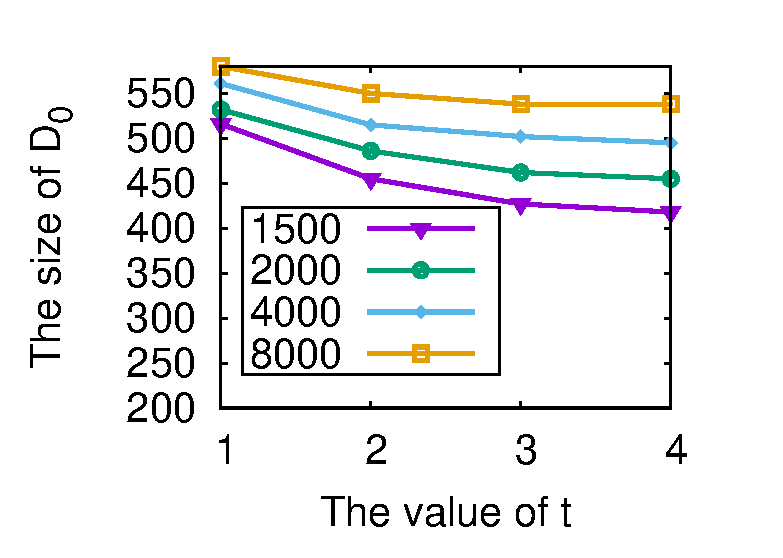
\includegraphics[width=0.5\textwidth]{1000-1-4.eps}}
	\subfigure[Network with 5000 nodes ]
	{\label{fig:e1:c}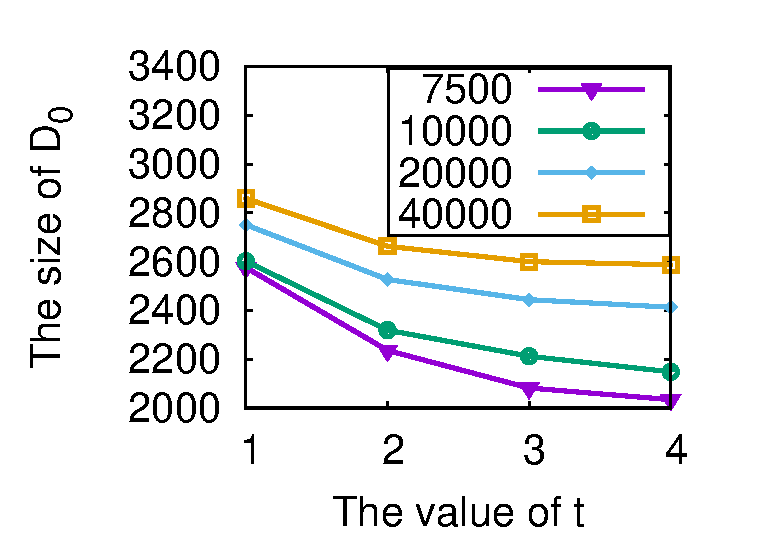
\includegraphics[width=0.5\textwidth]{5000-d0.eps}}
	\caption{The impact of average degree}
\end{figure}

\begin{figure}[!htb]
	\subfigure[Average degree is 3]
	{\label{fig:e1:d}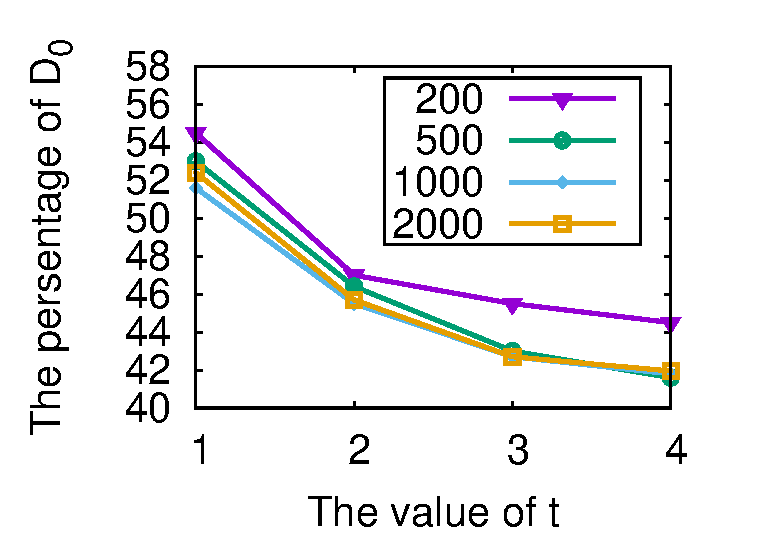
\includegraphics[width=0.5\textwidth]{200-500-3.eps}}
	\subfigure[Average degree is 4]
	{\label{fig:e1:e}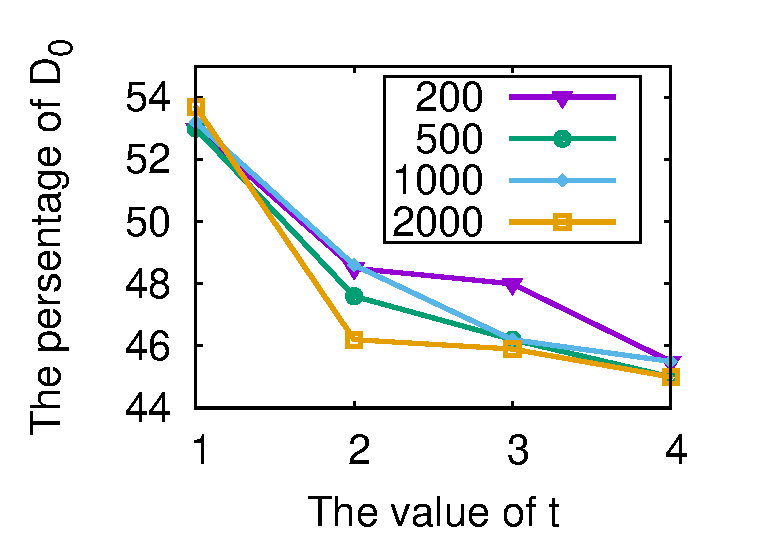
\includegraphics[width=0.5\textwidth]{200-500-4.eps}}
	\caption{The impact of number of nodes}
\end{figure}

\begin{figure}[!htb]
	\subfigure[The impact of number of nodes]
	{\label{fig:e1:f}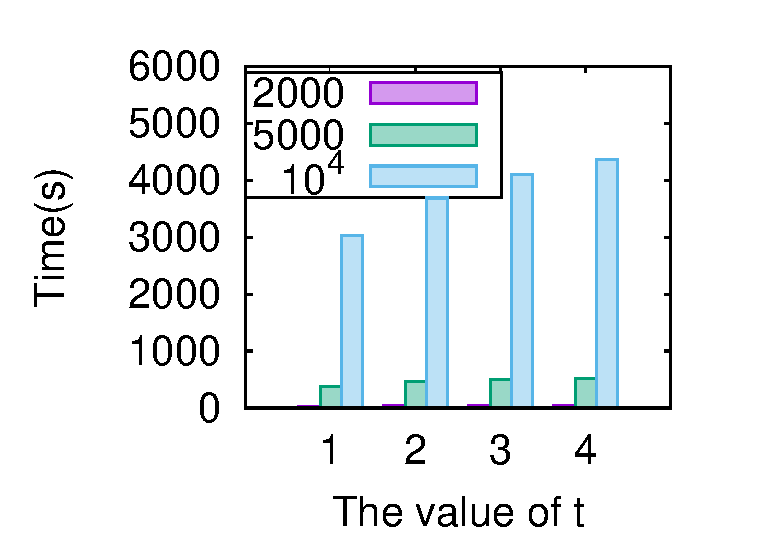
\includegraphics[width=0.5\textwidth]{2000-5000-10000.eps}}
	\subfigure[The impact of average degree]
	{\label{fig:e1:g}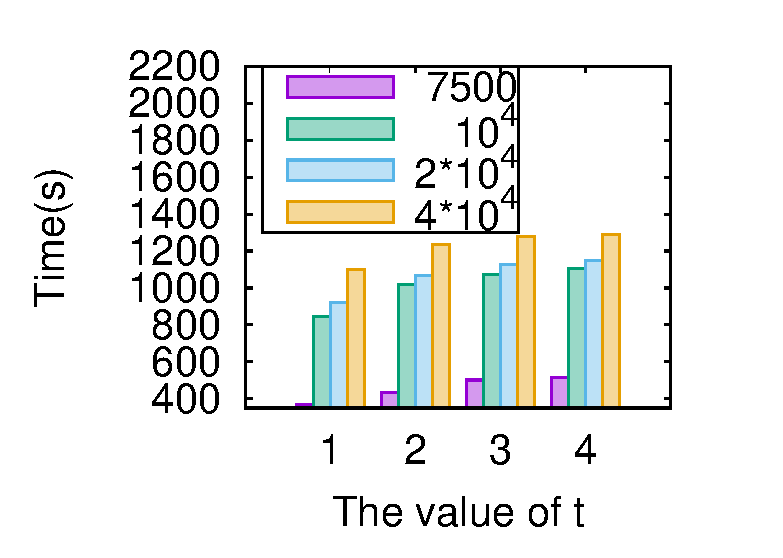
\includegraphics[width=0.5\textwidth]{5000-1-4.eps}}
	\caption{The impact of network size and average degree}
\end{figure}

\begin{figure}[!htb]
	\subfigure[Performance on real-world networks(The size of $D_0$)]
	{\label{fig:e2:a}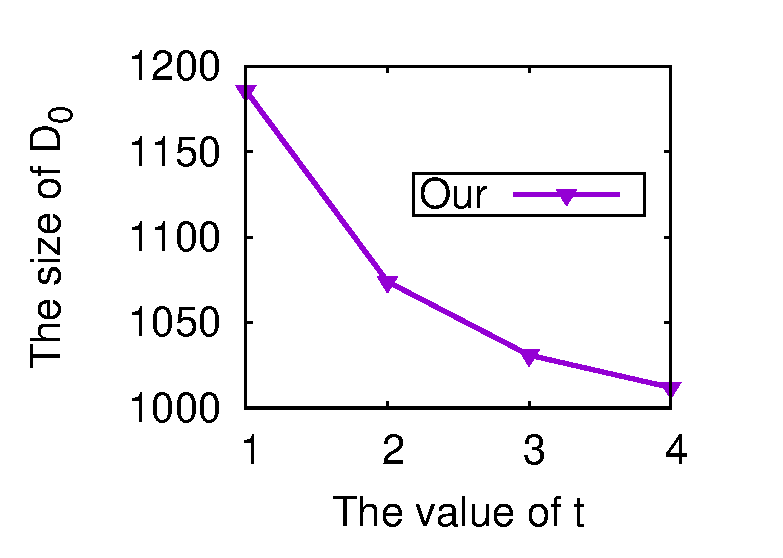
\includegraphics[width=0.5\textwidth]{real-d0.eps}} \hfil
	\subfigure[Performance on real-world networks(The running time)]
	{\label{fig:e2:b}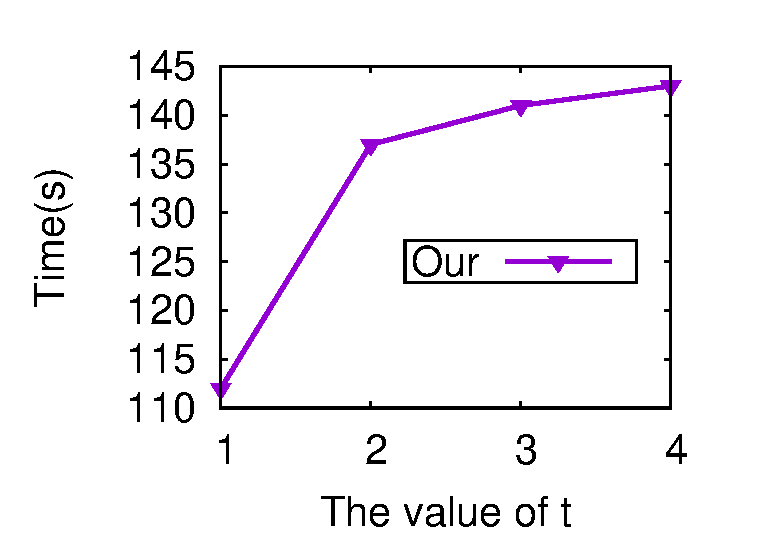
\includegraphics[width=0.5\textwidth]{real-time.eps}}
	\caption{Performance on real-world networks}
\end{figure}
\subsection{The impact of average degree}
%\vspace{-0.2cm}
To study the impact of average degree, we consider the networks with 1000 and 5000 nodes respectively, as shown in  Fig.\ref{fig:e1:b} and Fig.\ref{fig:e1:c}. For each network, we set the average degree as 3, 4, 8, and 16 and plot the relationship between the size of $D_0$ and the spread times $t$. Intuitively, the interdependence among the nodes is stronger in networks with large average degrees than those with small average degrees. We find that the size of $D_0$ does not continuously decrease dramatically when $t$ is larger than 4, so we just consider the situations with $t$ smaller than 4. Fig.\ref{fig:e1:b} and Fig.\ref{fig:e1:c} show that the size of $D_0$ in $V$ decreases as $t$ increases. On average, in the network whose average degree is 16, 2PIDS reduces by about 5.0\% compared with 1PIDS, while 4PIDS decreases by about 7.0\% compared with 1PIDS. However, on average, in the network whose average degree is 3, 2PIDS reduces by about 11.8\% compared with 1PIDS, while 4PIDS decreases by about 18.9\% compared with 1PIDS. When the average degree is much larger, the size of $D_0$ decreases more slowly.
In a word, for the network with the same number of nodes, our greedy algorithm performs well for both large average degree and small average degree. But the result obtained from the network with small average degree is much better.
%\vspace{-0.51cm}
\subsection{The impact of number of nodes}
%\vspace{-0.2cm}
%\textbf{The accuracy of the two algorithms}.
To study the impact of number of nodes, we consider the networks with 200, 500, 1000 and 2000 nodes respectively, as shown in Fig.\ref{fig:e1:d} and Fig.\ref{fig:e1:e}. In Fig.\ref{fig:e1:d} the average degree is 3 for each network and in Fig.\ref{fig:e1:d} the average degree is 4. We plot the relationship between the percentage of $D_0$ in $V$ and the spreading times $t$. In Fig.\ref{fig:e1:d}, the x-axis represents the times of spreading and the y-axis represents the percentage of $D_0$ in $V$. Apparently, the percentage of $D_0$ in $V$ decreases more or less due to the increasing spreading times $t$. For all of the above networks, the percentage of $D_0$ in $V$ decreases to about 40\% when $t$ grows to 4. In other words, we can choose a subset with only 40\% individuals of the society rather than the whole society to influence all the other individuals in 4 steps using our algorithm. The cost of choosing initial influence set is reduced largely. The situations of the 4 different networks are similar. Our greedy algorithm performs a little better in the networks with more nodes, since the average degree is the same. For example, when the average degree is 3, the interdependence of nodes is stronger in the network with 200 nodes. Generally speaking, the number of nodes does not affect the performance of our greedy algorithm much in condition that the interdependence among nodes is weak.
%\begin{figure}[!htb]
%	\centering
%	\subfigure[average degree is 3]
%	{\label{fig:e2:a}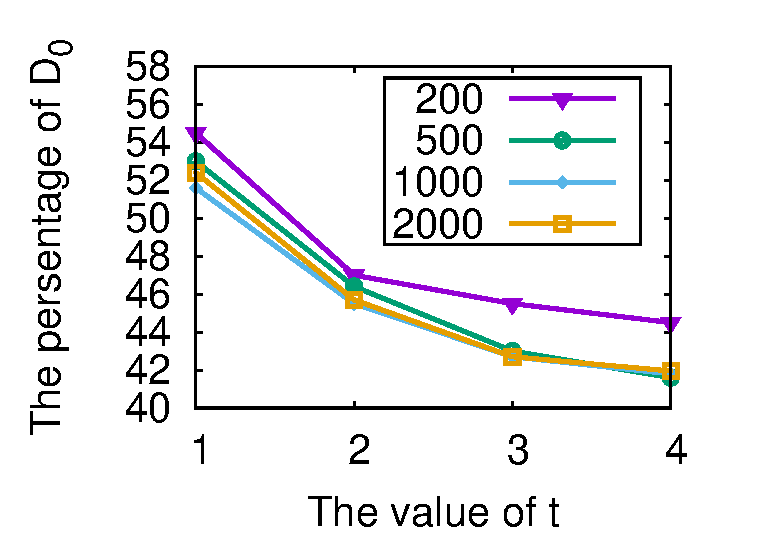
\includegraphics[width=0.23\textwidth]{200-500-3.eps}}
%	\hfil
%	\subfigure[average degree is 4]
%	{\label{fig:e2:b}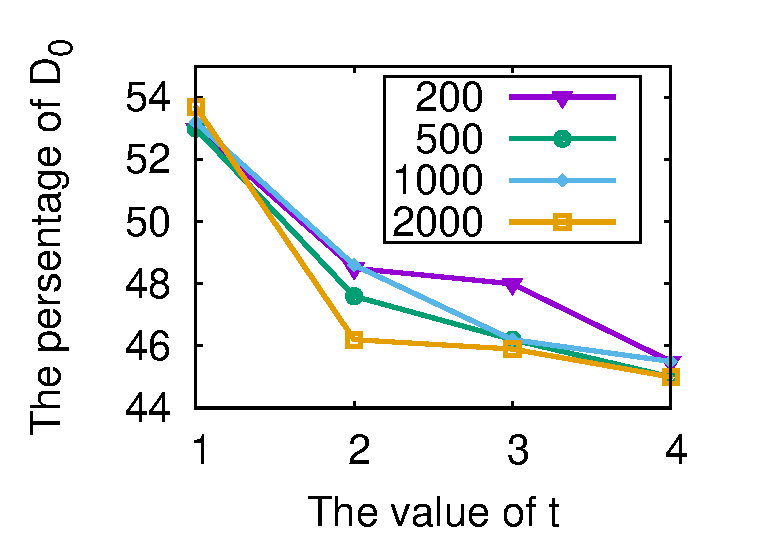
\includegraphics[width=0.23\textwidth]{200-500-4.eps}}
%	\caption{Impact of number of nodes.}
%	\label{fig:e2}
%\end{figure}
\subsection{The impact of network size and average degree on time efficiency}

To study the impact of nodes numbers on time efficiency of our greedy algorithm, we consider the networks with 2000, 5000 and 10000 nodes respectively, as shown in Fig.\ref{fig:e1:f}. The average degree of the network is set to 3. In Fig.\ref{fig:e1:f}, the x-axis represents the times of spreading and the y-axis represents the running time of our greedy algorithm. The histogram shows the relationship between running time and the times of spreading for the networks with different numbers of nodes. Visually, the running time of our algorithm increases slowly as the increasing spreading times increases. For example, consider the situation when $t$ is 3. For the network with 2000, 5000, and 10000 nodes, the cost of our algorithm is roughly 10, 500 and 4000 seconds respectively. To study the impact of average degree on time efficiency, we consider the network with 5000 nodes. The average degree is set to 3, 4, 6 and 12 respectively, as shown in Fig.\ref{fig:e1:g}. Intuitively, when the average degree is 3, the running time of our algorithm is less than 500 seconds, while the running time doubles when the average degree is larger. That is to say, our algorithm performs much better for sparse networks,  such as the disruption tolerant networks \cite{ShiNew/ZWLDC2014}.
For real-world social networks with millions of nodes, our algorithm is also feasible since a large network with weak interdependence among nodes can be divided into a sequence of strongly connected components, which contain much fewer individuals and can be served by our algorithm in an acceptable time bound.
%\begin{figure}[!htb]
%\centering
%\subfigure[a]
%{\label{fig:e3:a}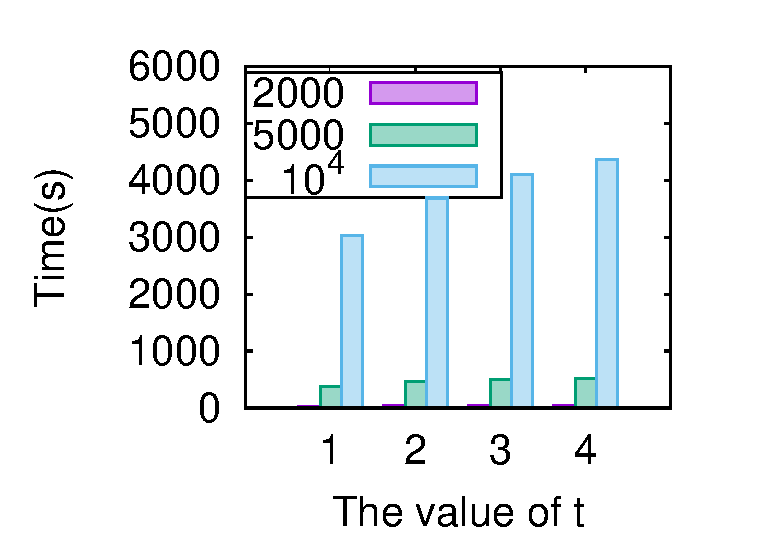
\includegraphics[width=0.23\textwidth]{2000-5000-10000.eps}}
%\subfigure[b]
%{\label{fig:e3:b}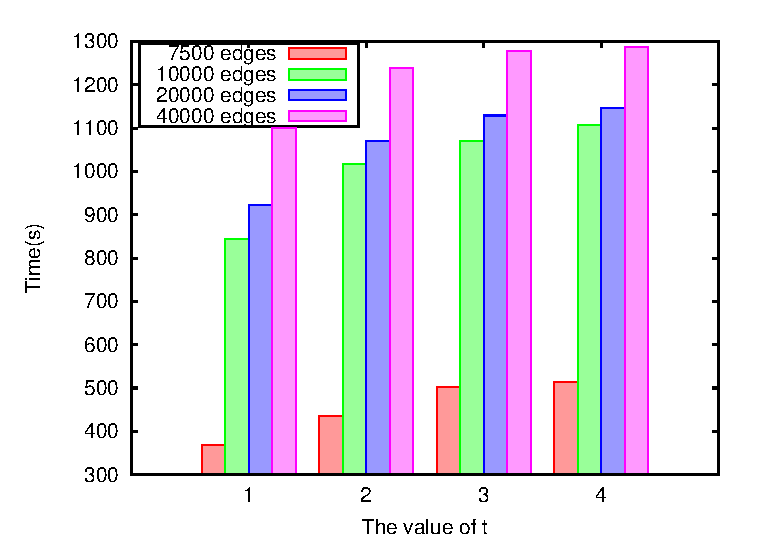
\includegraphics[width=0.23\textwidth]{5000-4-time.eps}} \hfil
%\caption{Performance in large networks.}
%\label{fig:e3}
%\end{figure}
\subsection{Comparison with the PIDS algorithm in \cite{WDC2011}}
The goal of the PIDS problem is to find a dominant set $D_0$ such that all the other nodes can be 
influenced by $D_0$ instantly, while the purpose of our tPIDS problem is to find a dominant set $D_0$ to
influence other individuals in a certain bounded time period. 
It is clear that the PIDS problem is a particular case of our tPIDS problem when $t$ is 1, that is, PIDS is equivalent to 1PIDS.
Then our greedy algorithm is also feasible for the PIDS problem. 
To compare our greedy algorithm with the algorithm in \cite{WDC2011}, we consider the network with 500
and 1000 nodes respectively and set the average degree to 3. As shown in Fig.\ref{fig:e1:h},
the x-axis represents the number of nodes in the graph and y-axis represents the size of the 
initial influence set $D_0$. Our result is almost the same as that of \cite{WDC2011}. 
However, the time efficiency of our algorithm is much better than that of \cite{WDC2011}. 
In Fig.\ref{fig:e1:i}, the x-axis represents the number of nodes in the graph and y-axis represents the running time
of the algorithm. In the network with 500 nodes, the running time of our algorithm is about 1 second 
while the running time of the algorithm in \cite{WDC2011} is over 22 seconds. 
In the network with 1000 nodes, the running time of our algorithm is about 8 seconds while the running time of the algorithm in \cite{WDC2011} is over 180 seconds. Our algorithm is almost 20 times faster than the algorithm in \cite{WDC2011}.
%\textbf{The difference between the two algorithms}.
\begin{figure}[!htb]
\subfigure[Comparison about the size of $D_0$]
{\label{fig:e4:a}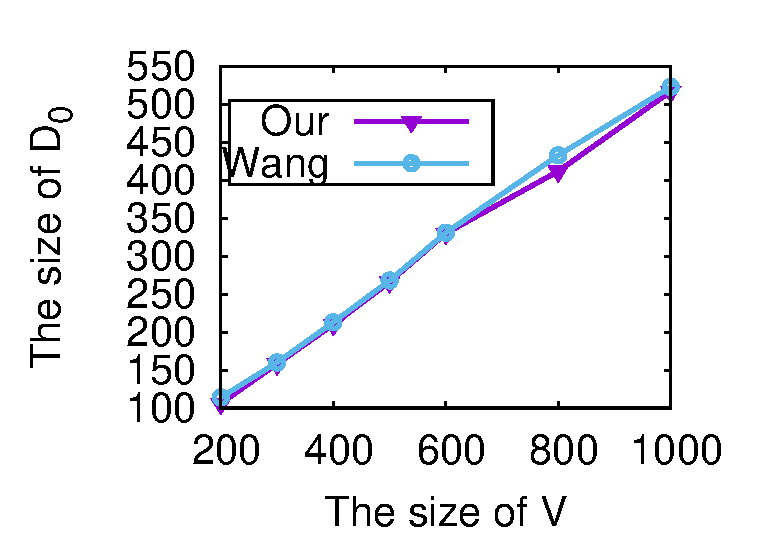
\includegraphics[width=0.5\textwidth]{our-wang.eps}} \hfil
\subfigure[Comparison about time ]
{\label{fig:e4:b}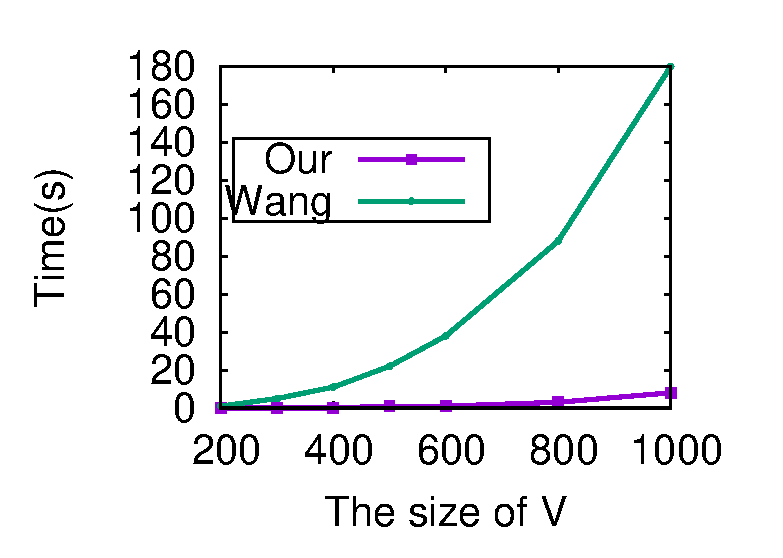
\includegraphics[width=0.5\textwidth]{our-wang-time.eps}}
\caption{Performance of the Proposed Algorithms.}
\label{fig:e4}
\end{figure}
\subsection{Performance on real-world networks}
In addition to simulated experiments, we conduct experiments based on realistic trace data sets provided by \cite{sju}. The given data set records the real-time longitude and latitude of 2370 taxies during half a month. Once two taxis appear in the same place at the same time, they will exchange some information. If the encounter time is greater than a constant, then we can consider that there is an edge between these two taxis. The taxi network contains 2370 nodes and 7631 edges, and the average degree is about 6.44. This taxi network is a mobile social network, which is a kind of social network and has been widely studied these years.  Fig.\ref{fig:e2:a} and \ref{fig:e2:b} shows the result of our algorithm on the given network.
As shown in Fig.\ref{fig:e2:a}, the percentage of 1PIDS, 2PIDS, 3PIDS and 4PIDS in the whole network is about 50.0\%, 45.3\%, 43.5\% and 42.7\% respectively. 2PIDS reduces by 9.4\% and 4PIDS reduces by 14.6\% compared with 1PIDS. That is, in order to send some information to all the 2370 taxis, one can choose about 42.7\% of the whole individuals. After 4 times of spread, all the taxis would receive the information. As shown in Fig.\ref{fig:e2:b}, the running time of 1PIDS, 2PIDS, 3PIDS and 4PIDS is 112s, 137s, 141s and 143s respectively. Evidently, the marginal utility of the running time decreases as the times of spread increases. The performance and time efficiency of our greedy algorithm are acceptable and feasible on the real-world networks.
\section{Conclusion}
This paper takes the first step towards the $t$ Positive Influence Dominating Set problem in social networks.
The $tPIDS$ problem takes the time factor, positive and group-to-individual interaction into account which is more practical in real social networks.
We build the $t$ SPREAD graph for a network and design a corresponding greedy algorithm. We also prove several significant theorems to support our algorithm.
We conduct extensive experiments on some randomly generated graphs and a real-world mobile social network. Our greedy algorithm works much better on loosely structured networks with roughly uniform degree of nodes.
The algorithm can reduce the percentage of initial nodes to about 40\%. 4PIDS reduces about 15\%-20\% compared with 1PIDS. Moreover, the running time of our algorithm is reasonable and acceptable.The experiment results show that our algorithm is effective and efficient. To some extent, as for the PIDS problem, our greedy algorithm performs better than the algorithm in \cite{WDC2011} especially on the aspect of effectiveness.
%\begin{acknowledgements}
%If you'd like to thank anyone, place your comments here
%and remove the percent signs.
%\end{acknowledgements}
% BibTeX users please use one of
%\bibliographystyle{spbasic}      % basic style, author-year citations
%\bibliographystyle{spmpsci}      % mathematics and physical sciences
\bibliographystyle{spphys}       % APS-like style for physics
\bibliography{ChengSocial}   % name your BibTeX data base

% Non-BibTeX users please use
%\begin{thebibliography}{}
%
% and use \bibitem to create references. Consult the Instructions
% for authors for reference list style.
%

%\end{thebibliography}

\end{document}
% end of file template.tex

